% po4a: environment astuce 
% po4a: environment alerte 
% po4a: environment links 
% po4a: environment tikzpicture  
% po4a: command -tikzstyle 
% po4a: command node [] [] {_}
% po4a: environment scope []
% po4a: command -usetikzlibrary {}
% po4a: command -def
% po4a: command -href {}{_}
% po4a: command -geometry {}
% po4a: command -arabic {}
% po4a: command -Roman {}
% po4a: command -alph {}
% po4a: command chemin {_}
\documentclass[a4paper,12pt]{report}
\usepackage[utf8]{inputenc}
%\usepackage[frenchb]{babel}
\usepackage[T1]{fontenc}
\usepackage{lmodern,textcomp}
\usepackage{graphicx}
%\usepackage{listings}
\usepackage{caption}
%\usepackage{fancybox}
\usepackage[pdftex]{hyperref}
%\usepackage{epsfig}
\usepackage{fancyvrb}
\usepackage{tikz}
\usetikzlibrary{shapes.geometric,backgrounds,fit,positioning,trees}
%\usetikzlibrary{arrows.meta,shapes.callouts}
\usepackage{wrapfig}
\usepackage{manfnt}
\usepackage{keystroke}
\usepackage{dingbat}
\usepackage{xcolor}
\usepackage{geometry}



\definecolor{reddebian}{rgb}{0.84314,0.03922,0.32549}
\definecolor{bluedane}{rgb}{0.09020,0.56863,1}
\definecolor{greendane}{rgb}{0.43137,0.60784,0.14510}
\def\purpledane{violet}

\hypersetup{%
  pdftitle={Xia},
  pdfauthor={Énuma Logiciel Libre},
  pdfsubject={Xia},
  pdfkeywords={Xia, logiciel libre, html5, Inkscape},
  colorlinks= true,
  linkcolor = greendane,
  urlcolor = bluedane
  }

% La dimension des marges
\geometry{hscale=0.7,vscale=0.85}

\title{Xia\\ Create HTML5 interactive images}

\renewcommand{\thechapter}{\arabic{chapter}}
\renewcommand{\thesection}{\Roman{section}}
\renewcommand{\thesubsection}{\alph{subsection}}

% pour unifier les indications relatives aux manipulation à effectuer dans les logiciels
% à modifier au besoin
\newcommand{\chemin}[1]{\texttt{\textcolor{reddebian}{#1}}}

% L'environnement alerte                        
\newsavebox{\boiteBrouillon}
\newcommand{\virageDanger}{\textdbend}

\newlength{\LargeurBouleAlerte}
\settowidth{\LargeurBouleAlerte}{
  
\begin{tikzpicture}
  \node{\virageDanger};
  \end{tikzpicture}
  }


% Style pour la boîte alerte
\tikzstyle{boitealerte}=[draw=red,rounded corners,inner xsep=1em,inner ysep=1ex]

% Style pour la boule alerte
\tikzstyle{boulealerte}=[circle,ball color=red,text=white] 

\newenvironment{alerte}{%
  \begin{lrbox}{\boiteBrouillon}% On sauve dans \boiteBrouillon le contenu
    \begin{minipage}{.8\linewidth}%  
      \color{red}%
      \setlength{\parskip}{1ex plus 0.2ex minus 0.2ex}%
}{%
    \end{minipage}%
  \end{lrbox}% Fin. Attention lrbox stocke du contenu sur 1 ligne (pas de paragrpahe)
  % La boîte peut être utilisée via \usebox{\boiteBrouillon}
  \vspace{1.5ex}%

  
\begin{tikzpicture}%
    \node [boitealerte] (cadre) {%
      \hspace{0.5\LargeurBouleAlerte}%
      \usebox{\boiteBrouillon}%
    };%
    \node [boulealerte] (alerte) at (cadre.west) {\virageDanger};%
  \end{tikzpicture}%
  \vspace{1.5ex}%
}        

% L'environnement astuce
\newcommand{\pouceOK}{\large\leftthumbsup}

\newlength{\LargeurBouleAstuce}
\settowidth{\LargeurBouleAstuce}{%
  \begin{tikzpicture}%
    \node{\pouceOK};%
  \end{tikzpicture}%
}

\tikzstyle{bouleastuce}=[circle,ball color=teal,text=white]

\tikzstyle{boiteastuce}=[draw=teal,rounded corners,inner xsep=1em,inner ysep=1ex]
                        
\newenvironment{astuce}{%
  \begin{lrbox}{\boiteBrouillon}% On sauve dans \boiteBrouillon le contenu
    \begin{minipage}{.8\linewidth}%
      \color{teal}%
      \setlength{\parskip}{1ex plus 0.2ex minus 0.2ex}%
}{%
    \end{minipage}%
  \end{lrbox}% Fin. Attention lrbox stocke du contenu sur 1 ligne (pas de paragrpahe)
  % La boîte peut être utilisée via \usebox{\boiteBrouillon}
  \vspace{1.5ex}%
  
\begin{tikzpicture}%
    \node [boiteastuce] (cadre) {%
      \hspace{0.5\LargeurBouleAstuce}%
      \usebox{\boiteBrouillon}%
    };%
    \node [bouleastuce] (astuce) at (cadre.west) {\pouceOK};%
  \end{tikzpicture}%
  \vspace{1.5ex}%
}    

% L'environnement links
\newcommand{\mainDroite}{\large\leftpointright}

\newlength{\LargeurBouleLinks}
\settowidth{\LargeurBouleLinks}{%
  \begin{tikzpicture}%
    \node{\mainDroite};%
  \end{tikzpicture}%
}

\tikzstyle{boulelinks}=[circle,ball color=\purpledane,text=white]

\tikzstyle{boitelinks}=[draw=\purpledane,rounded corners,inner xsep=1em,inner ysep=1ex]
                        
\newenvironment{links}{%
  \begin{lrbox}{\boiteBrouillon}% On sauve dans \boiteBrouillon le contenu
    \begin{minipage}{.8\linewidth}%
      \color{\purpledane}%
      \setlength{\parskip}{1ex plus 0.2ex minus 0.2ex}%
}{%
    \end{minipage}%
  \end{lrbox}% Fin. Attention lrbox stocke du contenu sur 1 ligne (pas de paragrpahe)
  % La boîte peut être utilisée via \usebox{\boiteBrouillon}
  \vspace{1.5ex}%
  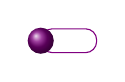
\begin{tikzpicture}%
    \node [boitelinks] (cadre) {%
      \hspace{0.5\LargeurBouleLinks}%
      \usebox{\boiteBrouillon}%
    };%
    \node [boulelinks] (links) at (cadre.west) {\mainDroite};%
  \end{tikzpicture}%
  \vspace{1.5ex}%
}    
